
\chapter{基于深度学习的骨髓血细胞检测算法设计与实现}
\section{引言}
骨髓血细胞形态学检查是血液疾病诊断的重要依据,主要通过人工镜检来完成,上述过程繁琐枯燥,可靠性差。
在骨髓血细胞自动化识别算法中,骨髓血细胞检测是将血细胞从涂片图像中定位并裁剪得到单一的血细胞图像,该过程是后续分类识别基础,
直接影响血液疾病诊断的结果,因此一直都是医学图像处理的热点研究方向之一。
目前基于深度学习的目标检测算法在很多领域都有广泛应用,如自动驾驶、安防监控、人脸识别、医学影像诊断等,其目的是定位或者跟踪相关目标。
本章提出了一种基于深度学习的改进RetinaNet骨髓血细胞自动化检测算法。

根据文献调研,目前血细胞检测主要是对血细胞图像中的红细胞、白细胞与血小板进行检测。
检测算法主要基于通用的深度学习目标检测算法,包括了单阶段检测算法与两阶段检测算法。
在两阶段方法中,通过区域举荐网络生成少量感兴趣区域,并将这些区域提取到的特征输入到后续的分类与回归分支中。
在单阶段算法中,如SSD、YOLO等网络直接将全部图像作为输入,学习类别概率与边界框位置。
两类方法各有优劣,本章第二节对这些方法进行阐述,并进行性能分析,最终选取性能较好的RetinaNet作为基线模型。

骨髓血细胞检测主要有如下三个难点:(1)相比外周血红细胞、白细胞、血小板三类血细胞检测,骨髓血细胞种类繁多、
形态丰富,尺寸大小不一。(2)在骨髓涂片制作过程中,由于染色剂与光照条件的变化,多个批次的数据存在着色彩差异。此外图像
背景复杂,存在较多成熟红细胞的干扰。(3)对于骨髓细胞增生活跃的切片,存在大量血细胞密集堆叠,边缘黏连,易导致漏检、错检等问题。
因此精准检测到骨髓血细胞是一项十分具有挑战性的课题。

针对上述难点,本章在第三节提出了一种改进RetinaNet网络,该方法提出了一种底向上的路径聚合网络结构,
缩短了底层与顶层特征之间的信息传递路径,提升了网络对位置特征的提取能力。此外探究了不同标签分配策略对检测性能的影响,
基于最优输运的标签策略可以提高密集区域的血细胞检测精度。此外我们比较了空洞卷积、深度可分离卷积、可变形卷积等卷积网络,以期实现速度与检测精度的更优均衡。
在骨髓血细胞数据集上的实验结果表明,本文提出的改进方法在检测准确率上有较大的提升,达到了较为先进的性能。

\section{基于深度学习的骨髓血细胞检测网络}

\subsection{快速区域卷积神经网络}
快速区域卷积网络(Faster-RCNN)是目标检测领域最为经典的两阶段检测器,其网络架构如图\ref{fig:faster_rcnn}所示,主要由
骨干网络特征提取器(BackBone)、区域举荐网络(Region proposal Network,RPN)与分类回归网络(R-CNN)这三部分组成。骨干网络为深度卷积神经网络,
用于图像特征提取。RPN网络在提取的特征图上快速生成区域坐标与相应前景分数,这些区域用于后续的分类与坐标回归。
R-CNN网络对于这些区域首先进行ROI池化(Region of Interest Pooling)将区域转换为特定大小的特征图,然后这些特征图会分别进入到
分类分支与回归分支,得到待检测目标的类别与位置信息。

\begin{figure}  
   \centering   
   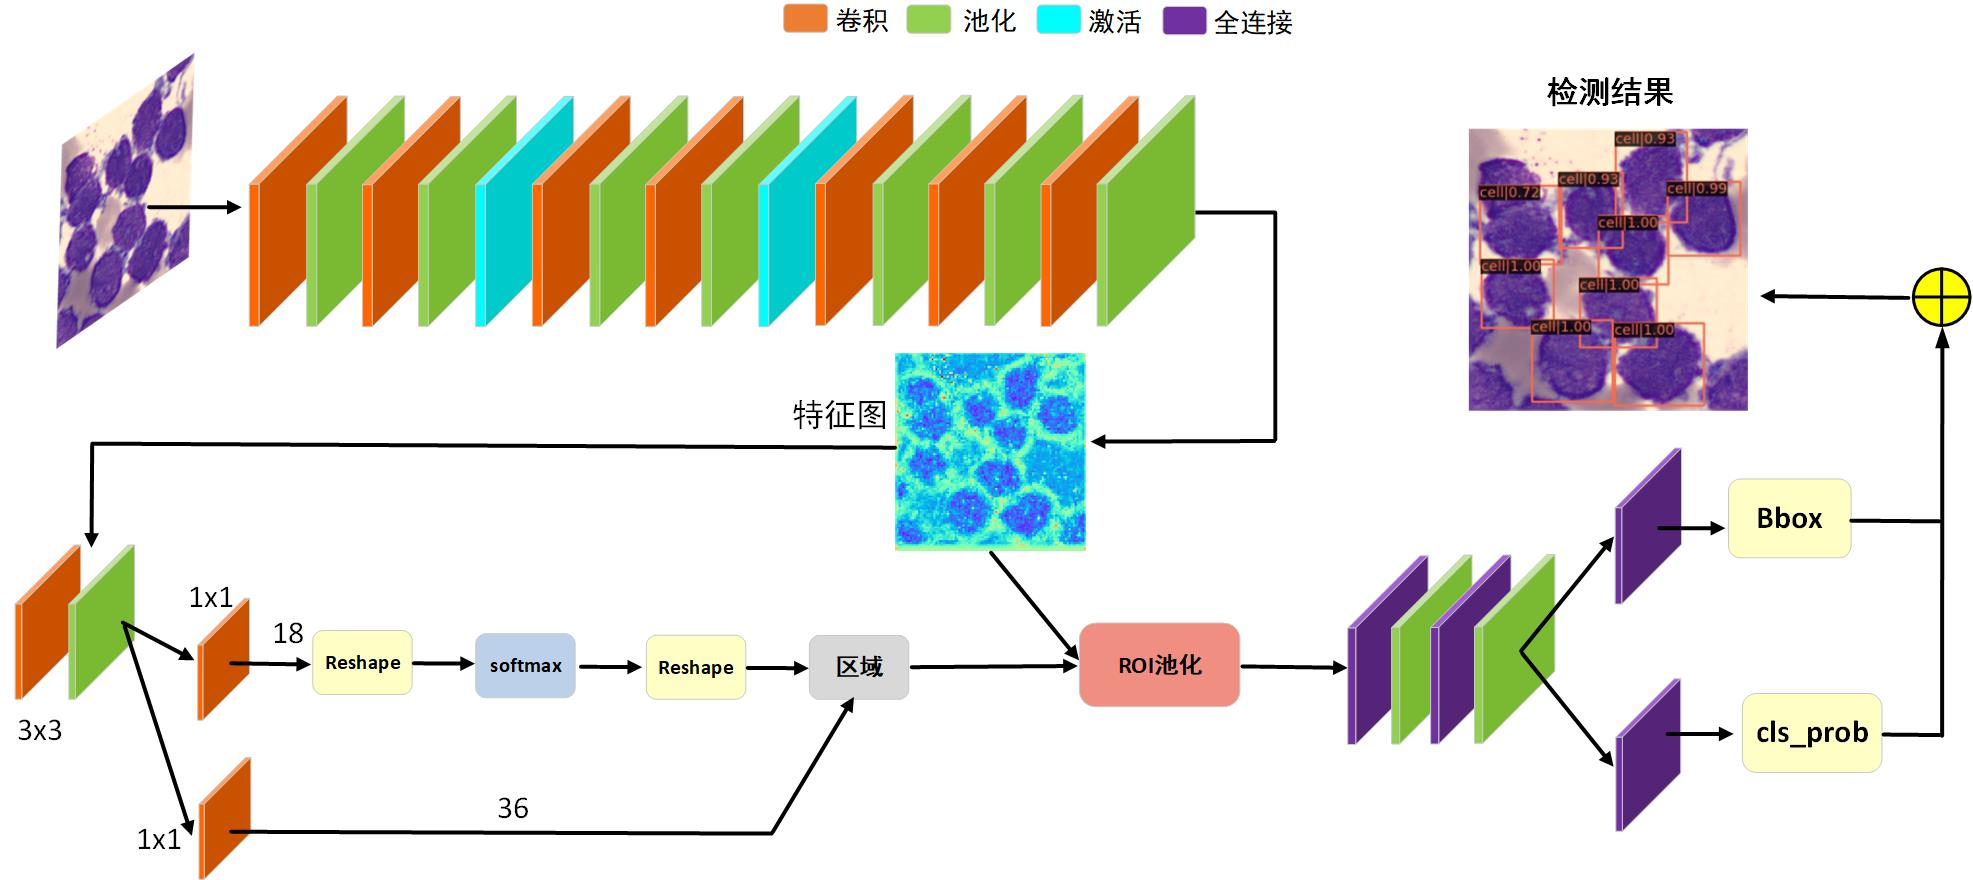
\includegraphics[width=0.9\linewidth]{faster_rcnn.jpg}   
   \caption{快速区域卷积神经网络结构示意图}   
   \label{fig:faster_rcnn} 
\end{figure}  

\subsubsection{骨干网络}
骨干网络是深度卷积神经网络的主体部分,用于提取图像抽象的语义特征,为后续任务提供图像的嵌入特征向量表示。
因此,骨干网络的性能对于整体网络性能具有很大的影响。常用的骨干网络有VGG、ResNet、DenseNet与Inception等,
其中ResNet是应用最为广泛的骨干网络,其特点是引入了残差模块,可以实现很深层的卷积网络。

综合考虑模型的精度、速度、参数量等因素,本节模型选择的骨干网络均为ResNet50,其结构如图~\ref{fig:resnet50}所示。
ResNet50总共由五个阶段(stage)构成,第一个阶段由一个$7\times7$的卷积组成,可视作对图像的预处理。
其余阶段均是由沙漏模块(BottleNeck)堆叠而成,第二到第五阶段分别有3、4、6、3个沙漏模块。若输入图像的大小为$224\times224\times3$
每经过一个stage,特征图的大小减小为原来的一半,通道数变为原来的两倍。五个阶段输出的特征图分别为$C_1, C_2, \dots, C_5$,
其中$C_5$特征图的大小为$7\times7\times2048$。最后特征图经过均值池化变为2048的向量,经过全连接层用于分类识别。

\begin{figure}      
  \centering       
  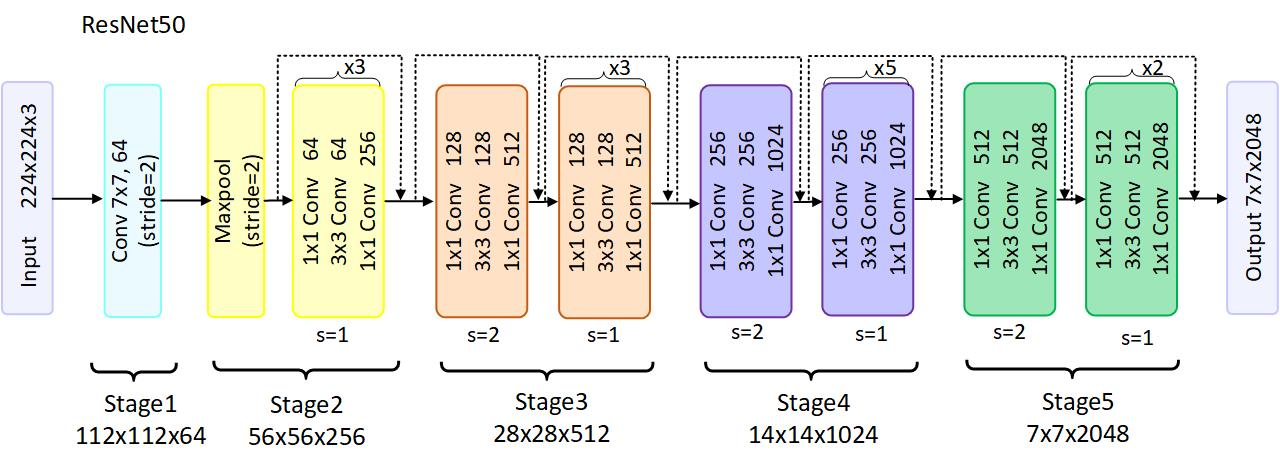
\includegraphics[width=0.9\linewidth]{resnet50.jpg}       
  \caption{ResNet50网络结构示意图}       
  \label{fig:resnet50}  
\end{figure}   

沙漏(BottleNeck)模块结构如图\ref{fig:bottleneck}所示,该网络第一个卷积层使用$1\times1$的卷积核来减少通道数量。
第二个卷积层的卷积核大小为$3\times3$,当stride为1时,特征图大小不变,stride=2时,特征图大小变为原来的一半。第三个卷积层采用$1\times1$卷积
恢复特征图的通道数。由于中间层的维度较小类似于沙漏,因此称为沙漏结构。该结构可以有效降低网络的参数量与计算量。
该结构还包括了一个残差模块,通过一个$1\times1$的卷积确保输入与输出的通道数相同后,在与输出直连相加。残差连接可以让网络更好的学习高层特征,
同时避免网络浅层部分梯度消失或爆炸等问题。图中BN为批归一化层、ReLU为激活函数。

\begin{figure}         
  \centering          
  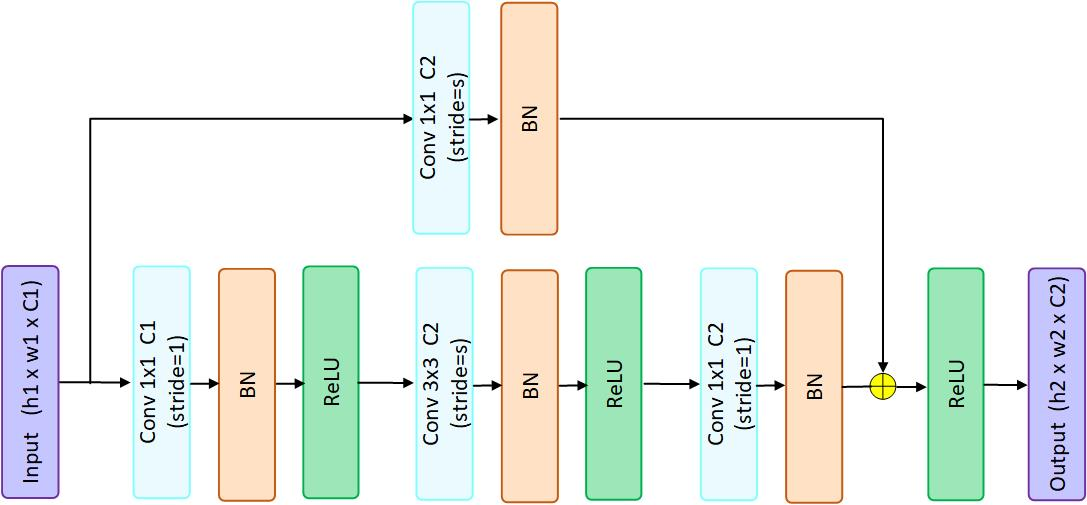
\includegraphics[width=0.7\linewidth]{bottleneck.jpg}          
  \caption{BottleNeck模块结构示意图}          
  \label{fig:bottleneck}   
\end{figure}    

\subsubsection{特征金字塔网络}

特征金字塔网络(Feature Pyramid Network,FPN)主要用来解决多尺度的目标检测问题。骨干网络特征提取器输出不同尺度的特征图,这些特征图的感受野不同。
高层特征图感受野比较大,用来检测大尺寸目标,浅层的特征图感受野较小,用来检测小尺寸目标。
但是浅层特征图的表达能力较弱,通常只有纹理、边缘形状、明暗等细节信息,而高层特征图则包含更加丰富的全局信息。
为解决浅层网络特征表达能力有限的问题,引入了特征金字塔网络。该网络将顶层特征逐级向下传递并与浅层特征融合,
使得浅层特征可以同时兼顾细节与整体具有更加丰富的特征表达。ResNet50骨干网络构建特征金字塔的结构如图~\ref{fig:fpn}所示。
图中$C_1,C_2 \cdots C_5$为ResNet骨干网络生成的不同尺度特征图,相邻两个阶段的特征图在尺寸上为二倍缩放的关系。
自顶向下的融合过程经过上采样与通道调整使得特征图的尺寸一致后再相加融合。以$P_4$特征图的生成为例,$P_5$由$C_5$特征图经过$1\times1$、通道数为256的卷积层得到。
$P_5$经过二倍上采样(由反卷积实现)与$C_4$经过$1\times1$、通道数为256的卷积的结果相加得到$P_4$。其他特征图同样由上述过程生成。
最后FPN使用$3 \times 3$卷积对融合后的特征图进行平滑处理消除直接相加可能导致的融合不充分问题。至此,完成了特征金字塔的构建。

\begin{figure}            
  \centering             
  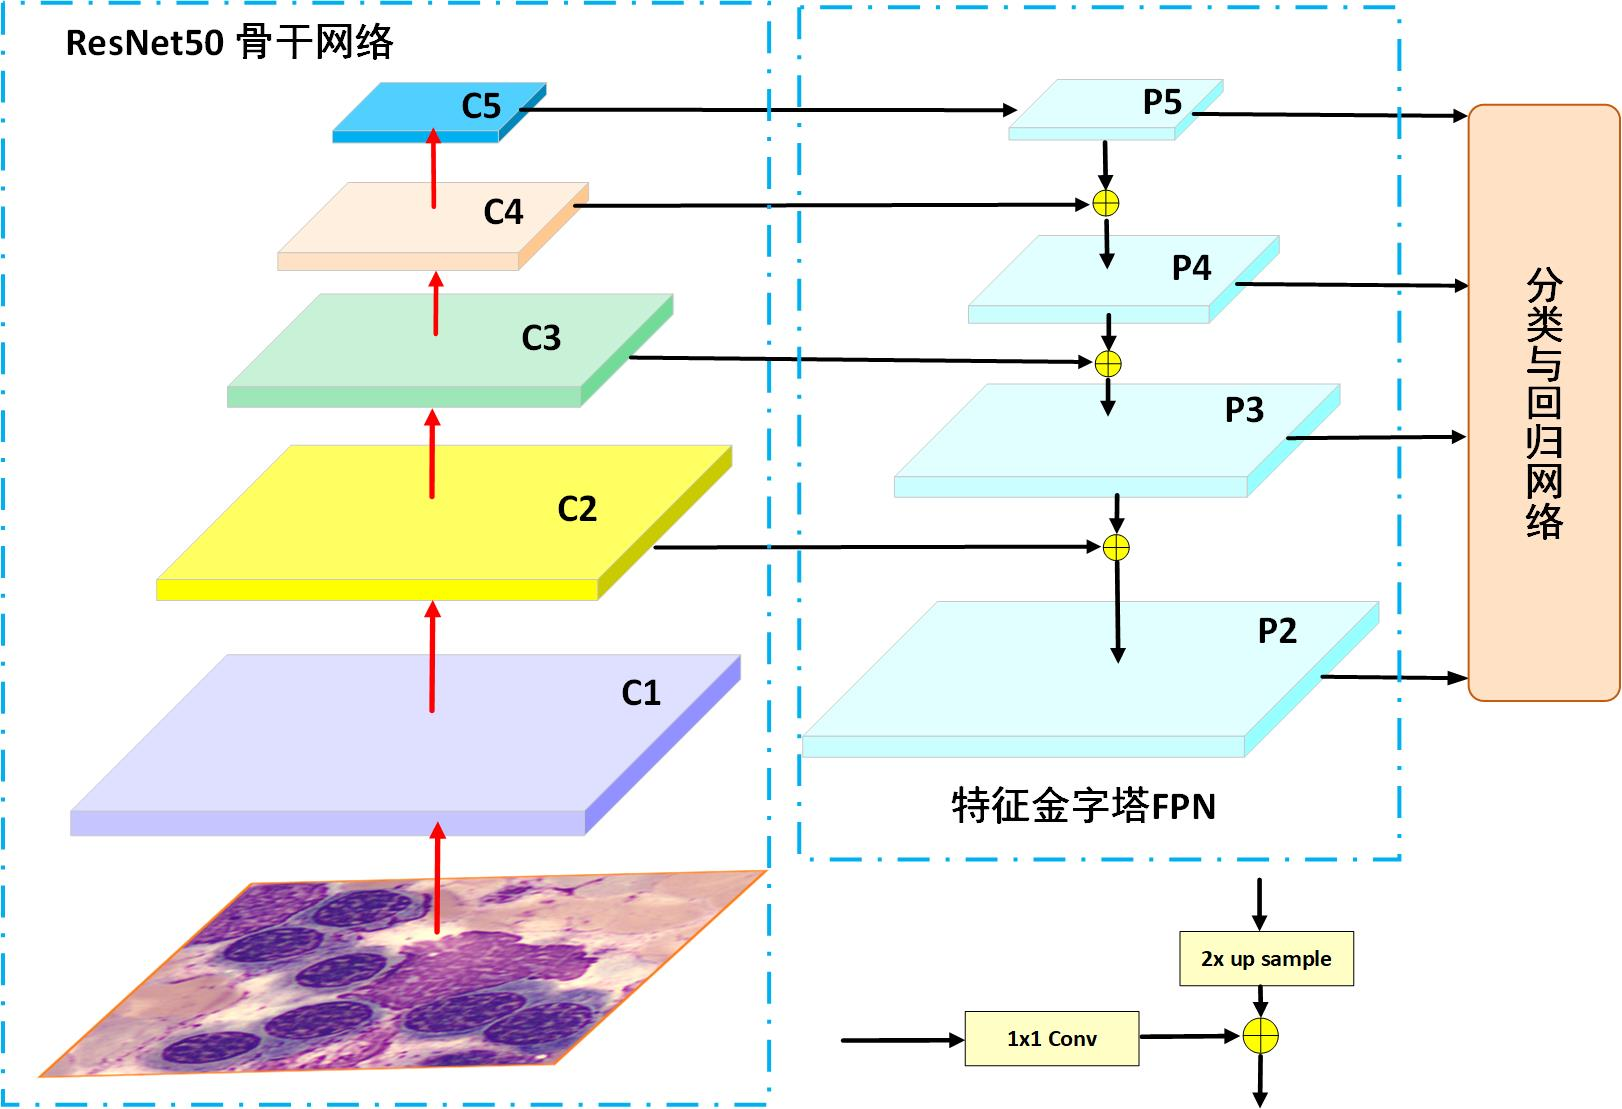
\includegraphics[width=0.65\linewidth]{fpn.jpg}             
  \caption{特征金字塔网络结构示意图}             
  \label{fig:fpn}    
\end{figure}    

\subsubsection{区域举荐网络}

区域举荐网络

\subsubsection{分类与回归网络}

\subsection{单阶段RetinaNet检测网络}
\subsection{通用目标检测网络性能对比}

\section{改进的RetinaNet骨髓血细胞检测网络}
\subsection{路径聚合网络}
\subsection{基于最优输运的标签分配策略}
\subsection{卷积模块}
\section{算法实现与实验结果分析}
\subsection{实验环境}

\textbf{1)数据集介绍}

骨髓血细胞图像来自邃蓝智能科技(上海)有限公司合作医院提供,首先采用第2.1小节阐述的主动学习标注策略进行边界框的标注。
我们总共标记了6821张血细胞图像,训练集与测试集按照4:1的比例进行随机划分,训练集包含了5456张图像,测试集包含了1365张图像。
通常每个图像中包含1到10个有核血细胞,数据集总共标记了11352个血细胞,训练集有9065个血细胞,测试集有2287个血细胞。数据集的分布如
表~\ref{table:cell_detect}所示:

\begin{table}
  \caption{骨髓血细胞检测数据集分布}   
  \centering 
  \label{table:cell_detect}
  \begin{tabular}{ccccc}
    \toprule[2pt]
    序号 & 类别名  &  类别简写 & 训练集数量 & 测试集数量 \\
    \midrule[1.5pt] 
    1 & 原始细胞 & Prim & 1856 & 467 \\ 
    2 & 淋巴细胞 & Lym & 996 & 226   \\ 
    3 & 单核细胞 & Mono & 206 & 52   \\ 
    4 & 浆细胞 & Plas & 272 & 70   \\ 
    5 & 红细胞 & Red & 1880 & 503   \\ 
    6 & 早幼粒细胞 & Promy & 357 & 107   \\ 
    7 & 嗜中性中幼粒细胞 & Myelo & 701 & 150   \\ 
    8 & 嗜中性晚幼粒细胞 & Late & 503 & 144   \\ 
    9 & 嗜中性杆状核细胞 & Rods & 998 & 241   \\  
    10 & 嗜中分叶核细胞 & Lobu & 821 & 195   \\  
    11 & 嗜酸性粒细胞 & Eosl & 475 & 132   \\  
    \hline
    总计 &   &   & 9065 & 2287 \\
    \bottomrule[2pt]      
  \end{tabular} 
\end{table}
\subsection{消融实验}
\subsection{实验结果与分析}
\section{小结}


